

\section{Automatischer Löser Wechsel}

Im Kaptiel \ref{} wurde die Vor- und Nachteile der Impliziten und expliziten Differenzialgelichungslöser 
vorgestellt.

In diesem Kapitel wird untersuch wie die vorteile beider verfaheren so miteinander verbunden 
werden können, dass das projekt so wohl mit einer hohen genauichkeit, als auch einer verträglichen laufzeit
ausgeführt werden kann.
Wie bereits gezeigt wurde, liefern die unterschiedlichen löser zu unterschiedlichen zeitpunkten
unterschiedlich gute ergebnisse.
Das \textit{DifferentialEquations.jl} Projekt bietet dafür die möglichkeit automatisch 
zwischen verschiedenen lösungsverfahren zuwechseln.

Dies geschieht meist abhängig von aktuellen Fehler, es können aber auch eigene Kriterien entwickelt werden.

Dabei ist jedoch zu beachten das dies nicht mit allen Verfahren möglich ist.

So ist es zum beispiel nicht möglich den impliziten mit dem expliziten euler zu verbinden.

Deshalb wird im folgendem der \textit{Tsit5} mit dem \textit{Rosenbrock23} verbunden. Dieser Algorithmus wird im folgendem als AutoTsit5 bezeichnet.

Dessenlaufzeit kann stark varieren. Je nach problem kann die laufzeit zwischen ein paar sekunden und
ein paar studen sein.

In den für dieses Kaptiel berechneten trajectorien, war die geringste laufzeit 19s und die längste 2h.

Die genaue laufzeit hängt sehr stark von den benötigten fehler toleranzen und der problem größe ab.

Im folgenden wird das bereits genannte verfahren mit dem expliziten euler verglichen.

\begin{figure}[h]
    \centering
    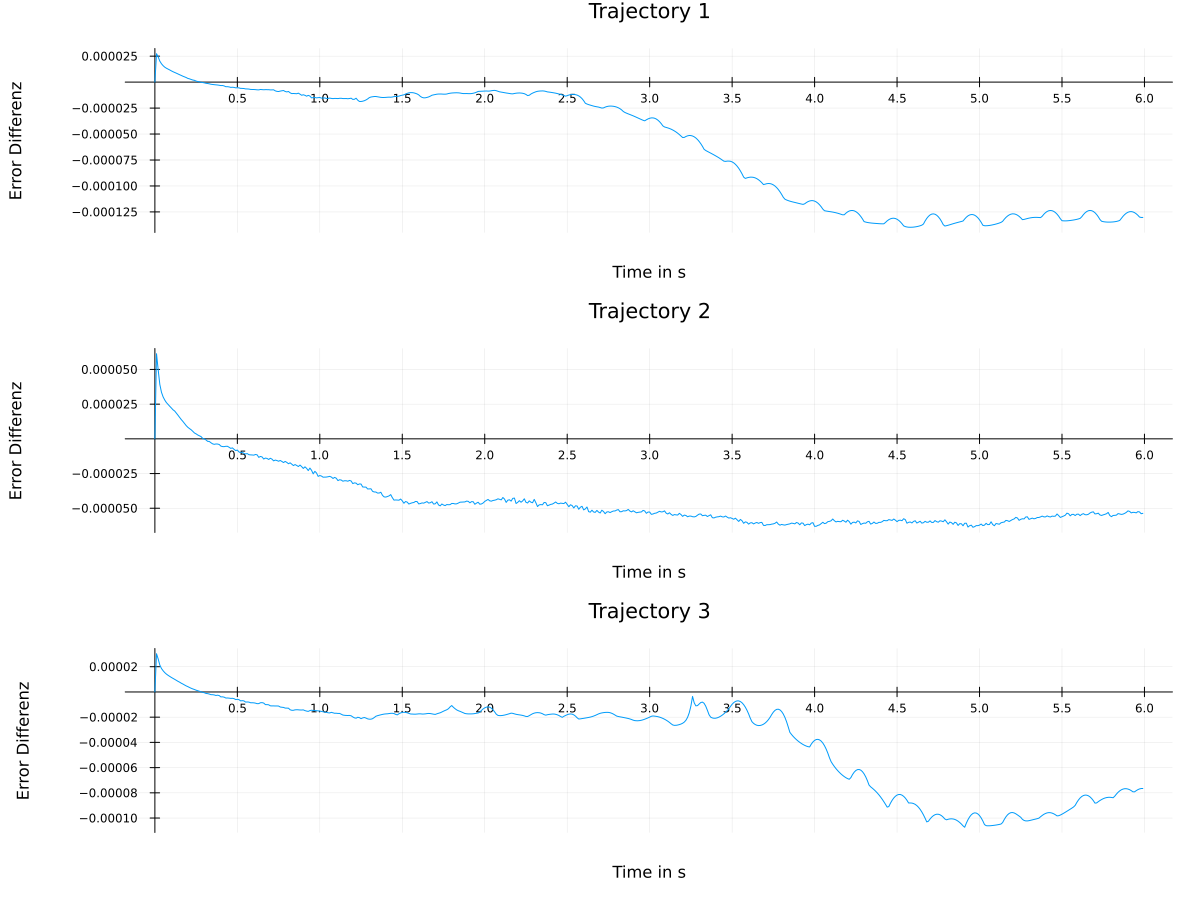
\includegraphics[width=\textwidth]{Data/03_Ergebnisse/autoswitching/errors_explizit_composit.png}
    \caption{Vergleich mit Explizit Algorithm}
    \label{fig:vergleichexplizit}
\end{figure}

In der Grafik \ref{fig:vergleichexplizit} wird die differenz zwischen dem Expliziten Euler und dem AutoTsit5 verglichen.

In den ersten 0.5 sekunden ist die differenz positiv, dies bedeutet, dass
der Explizite euler bessert.

Danach liefert der AutoTsit dann ein konstant besseres ergebniss.




\begin{figure}[h]
    \centering
    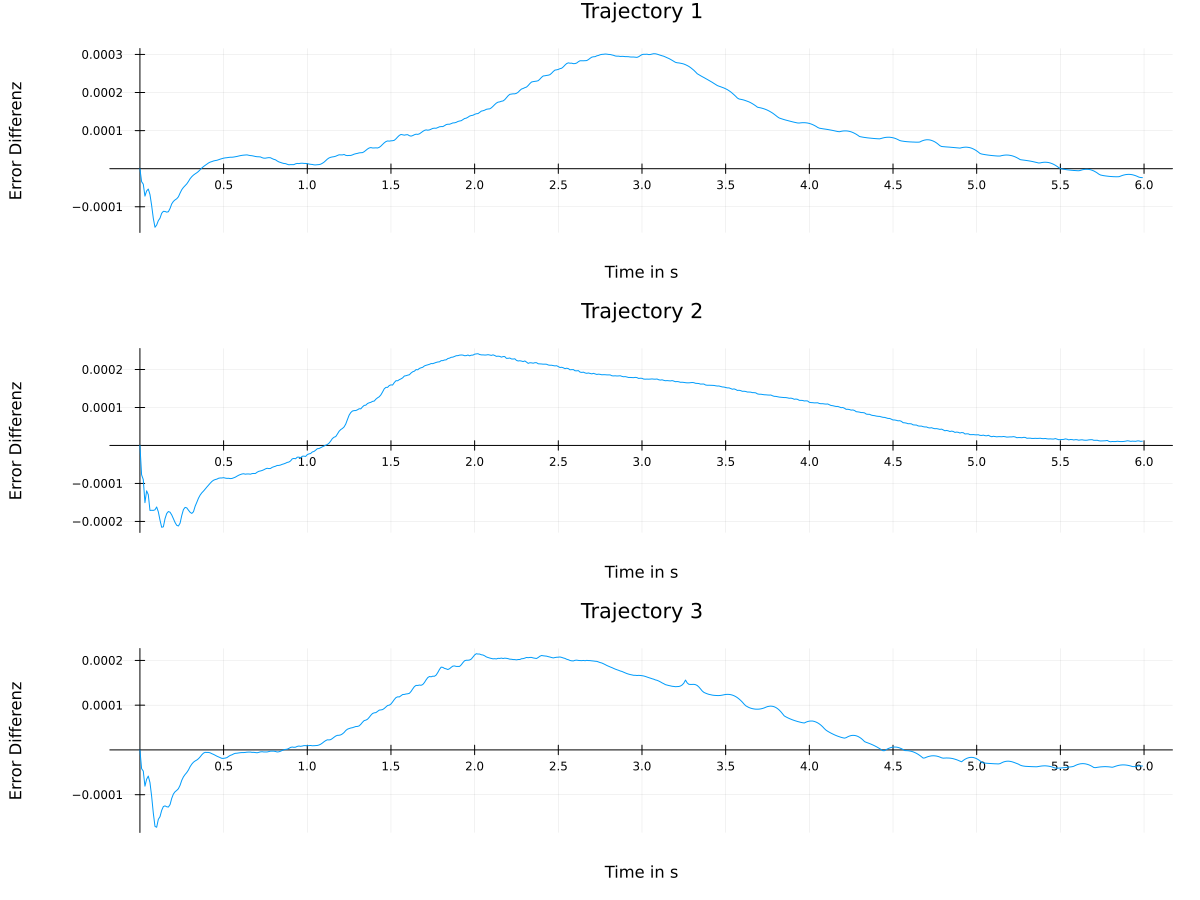
\includegraphics[width=\textwidth]{Data/03_Ergebnisse/autoswitching/errors_implizit_composit.png}
    \caption{Vergleich mit Implizit Algorithm}
    \label{fig:vergleichimplizit}
\end{figure}

In der Graphik \ref{fig:vergleichimplizit} wird beobachtet,
dass der AutoTsit5 am Anfang einbessers ergebniss liefert.

Nach etwa 1 sekunde wird dann der Implizite Euler besser.

Besonders ist vorallem das der Unterschiede zwischen beiden verfahren gegen ende sich sehr stark null annähert und bei zwei der drei trajektorien gegen ende wieder ein bessers ergebniss liefert.

Dies lässt vermuten das der AutoTsit bei längeren trajektorien, ein sehr gutes ergebniss liefert.











